\documentclass[12pt,addpoints]{exam}

\usepackage{tikz}
\usepackage{tkz-tab}
\usepackage[margin=2cm]{geometry}
\usepackage{amsmath}
\usepackage{multicol}
\usepackage{frenchmath}
\usepackage{siunitx}

\begin{document}

\begin{center}
    \Huge{Interrogation sur les inégalités et les inéquations}
\end{center}

\begin{questions}

\question[3] Recopier et compléter par le bon signe, en justifiant.
\vspace{-0.5cm}
\begin{multicols}{3}
\begin{parts}
    \part
    \begin{minipage}{0.3\linewidth}
    \begin{align*}
        3x &\infeg 9 \\
        \Leftrightarrow x &~?~ 3
    \end{align*}
    \end{minipage}
    \part
    \begin{minipage}{0.3\linewidth}
    \begin{align*}
        x + 5 &\supeg 3 \\
        \Leftrightarrow x &~?~ -2
    \end{align*}
    \end{minipage}
    \part
    \begin{minipage}{0.3\linewidth}
    \begin{align*}
        -2x &\infeg 8 \\
        \Leftrightarrow x &~?~ -16
    \end{align*}
    \end{minipage}
\end{parts}
\end{multicols}

\question[4] Résoudre les inéquations suivantes
\begin{multicols}{2}
\begin{parts}
    \part $7x+ 12 \infeg 9 - 2x$
    \part $-3x - 7 \supeg -7x -27$
\end{parts}
\end{multicols}


\question[4] Sachant que $-2 \infeg a \infeg 5$ et $-1 \infeg y \infeg 4$, encadrer les nombres suivants
\begin{multicols}{4}
\begin{parts}
    \part $3x + 4y$
    \part $2x + 5y$
    \part $-3y$
    \part $2x - 3y$
\end{parts}
\end{multicols}



\question[4] Résoudre les inéquations suivantes
\begin{multicols}{2}
\begin{parts}
    \part $(2x+3)(-x-2) \supeg 0$
    \part $\dfrac{(3x+2)(-x+7)}{3x-4} \infeg 0$
\end{parts}
\end{multicols}

\medskip

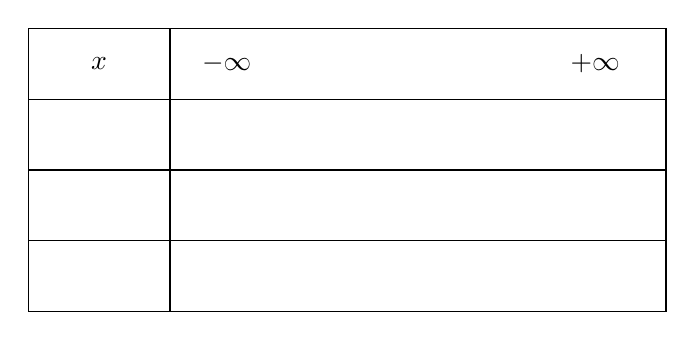
\begin{tikzpicture}[scale=0.9]
    \draw (0,0) rectangle (9,-1);
    \draw (0,-1) rectangle (9,-2);
    \draw (0,-2) rectangle (9,-3);
    \draw (0,-3) rectangle (9,-4);
    \draw (0,0) rectangle (2,-4);
    \node at (1,-0.5) {{$x$}};
    \node at (2.8,-0.5) {$-\infty$};
    \node at (8,-0.5) {$+\infty$};
\end{tikzpicture}\hfill
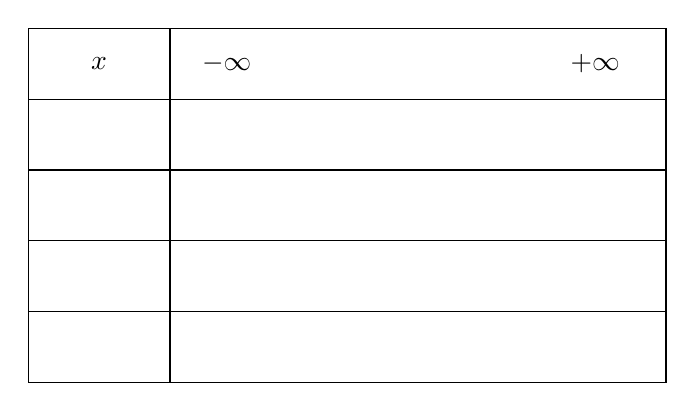
\begin{tikzpicture}[scale=0.9]
    \draw (0,0) rectangle (9,-1);
    \draw (0,-1) rectangle (9,-2);
    \draw (0,-2) rectangle (9,-3);
    \draw (0,-3) rectangle (9,-4);
    \draw (0,-4) rectangle (9,-5);
    \draw (0,0) rectangle (2,-5);
    \node at (1,-0.5) {{$x$}};
    \node at (2.8,-0.5) {$-\infty$};
    \node at (8,-0.5) {$+\infty$};
\end{tikzpicture}

\question[5] Soit la figure suivante composée de deux triangles $ABM$ et $CDM$.

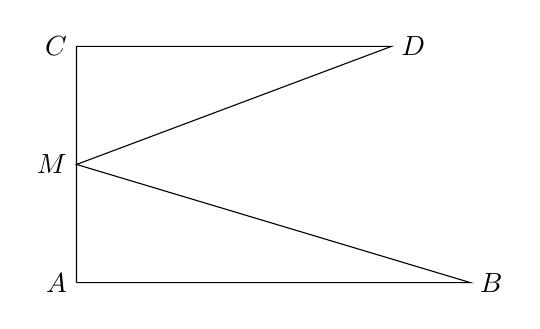
\begin{tikzpicture}
    \coordinate (A) at (0,0);
    \coordinate (B) at (5,0);
    \coordinate (C) at (0,3);
    \coordinate (D) at (4,3);
    \coordinate (M) at (0,1.5);
    \draw (A) -- (B) -- (M) -- (D) -- (C) -- (A);
    \node[left] at (A) {$A$};
    \node[right] at (B) {$B$};
    \node[left] at (C) {$C$};
    \node[right] at (D) {$D$};
    \node[left] at (M) {$M$};
\end{tikzpicture}

Nous savons que $AB = \qty{5}{\cm}$, $CD= \qty{4}{\cm}$ et $AC = \qty{3}{\cm}$. Le point $M$, quant à lui, n'a pas de position fixe, il peut se déplacer sur le segment $[AC]$. La distance $AM$ est donc variable.\\
Dans cet exercice, nous cherchons à connaître les positions du point M pour lesquelles l'aire du triangle $CDM$ est supérieure à celle du triangle $ABM$.

\begin{parts}
    \part Montrer que ce problème revient à étudier l'inéquation $\dfrac{12 - 4x}{2} \supeg \dfrac{5x}{2}$
    \part Résoudre cette inéquation. Pourquoi $x$ ne peut être supérieur à 3 ?
\end{parts}

\end{questions}
\end{document}